\documentclass[a4paper, 12pt]{mcshw}
\begin{document}
\Letsmaketitle{3}
\begin{enumerate}
    \item 
        \begin{enumerate}
            \item 
                What is the surface area of a unit cube in d-dimensions?
                \begin{solution}
                    The d-dimensional cube has $2d$ faces, and each face has area 1, so the surface area is $2d$.
                \end{solution}
            \item
                Is the surface area of a unit cube concentrated close to the equator, define here as the hyperplane $\{x: \sum\limits_{i = 1}^{d}x_i = \frac{d}{2}\}$, as is the case with the sphere?
                \begin{solution}
                    Yes.

                    Suppose we are uniformly generating points on the surface of the cube. Then to prove the surface area is concentrated close to the equator, we only need to prove that the distance between the random generated point the the hyperplane is almost always near zero. 
                    
                    To show this, let $p$ be a random generated point, having coodinates $x_1$ to $x_d$, $X$ be a random variable, $X = \sum_{i = 1}^{d}xi$. And $d$ be the distance between $l$ and the hyperplane representing the equator. Then we have $X = \sqrt{d}l$. So what we really need to prove is the random variable $X$, which takes value from $0$ to $d$, is almost always near $\frac{d}{2}$.

                    First we notice that, due to the symmetrical properties, $E(X) = \frac{d}{2}$.
                Then we need to calculate $Var(x)$. But the $d$ coordinates are not independent, so we should do a little bit transformation. Every time we generate a point. We can consider the generation in such a way. First we choose one dimension, let its coodinate to be $0$ or $1$, with equal probability. Then let the rest $d - 1$ coodinates take value uniformlly from $0$ to $1$. At last we change the dimension considered first to the first coodinate, this doesn't change the value of $X$. In this way, the $d$ coodinates are independent, and 
                \begin{align*}
                    Var(X) &= Var(x_1) + \sum\limits_{i = 2}^{d}x_i\\
                    &= \frac{1}{4} + (d - 1)\int_{0}^{1}(x - \frac{1}{2})^2 dx\\
                    &= \frac{1}{4} + (d - 1)\frac{1}{12}\\
                    &= \frac{d}{12} + \frac{1}{6}
                \end{align*}
                Then according to the Chebyshev's Inequality, we have
                $$p(|X - E(X)| \geq \epsilon) \leq \frac{Var(X)}{\epsilon^2}$$
                this means
                $$p(|X - \frac{d}{2}| \geq \epsilon) \leq \frac{\frac{d}{12} + \frac{1}{6}}{\epsilon^2} \leq \frac{d}{4\epsilon^2}$$
                The distance between the equator and the farthest point from it is $\frac{\sqrt{d}}{2}$. Now as the dimension goes higher and higher, we consider a slice near equator of length $c\frac{d}{2}$, where $c$ can be a quite small number. This slice takes a fixed proportion of the height of the north pole from the equator, where the north pole is the farthest point from the equator we have mentioned before. Since a point's distance from equator equals $\frac{X - E(X)}{\sqrt{d}}$, we should let $\epsilon$ be $c\frac{\sqrt{d}}{2}$ times $\sqrt{d}$, which is $\frac{d}{2}$, then the equation becomes
                $$p(|X - \frac{d}{2}| \geq c\frac{d}{2}) \leq \frac{1}{c^2 d}$$
                This means, for very large d, the surface area is always near the equator.
                \end{solution}
        \end{enumerate}
    \item
    Generate 20 points uniformly at random on a 1,000-dimensional sphere of radius 100. Calculate the distance between each pair of points. Then project the data onto subspaces of dimension $k = \{100, 50, 10, 5, 4, 3, 2, 1\}$ and calculate the sum of squared error between $\frac{k}{d}$ times the original distances and the new pair wise distances for each of the above values of $k$.
    \begin{solution}
        Since what really matters is the relative error, so I calculate the sum of squared relative errors. A mathematica code is shown as below. 
        \begin{center}
            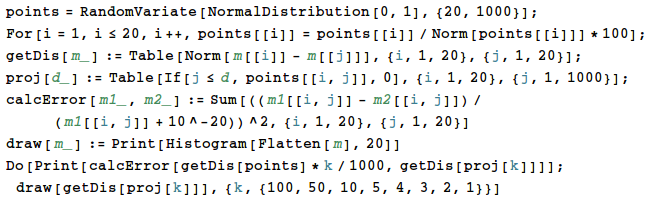
\includegraphics[height=4.5cm]{1.png}
        \end{center}
        When $k = 100$, the answer is 1.04293
        \begin{center}
            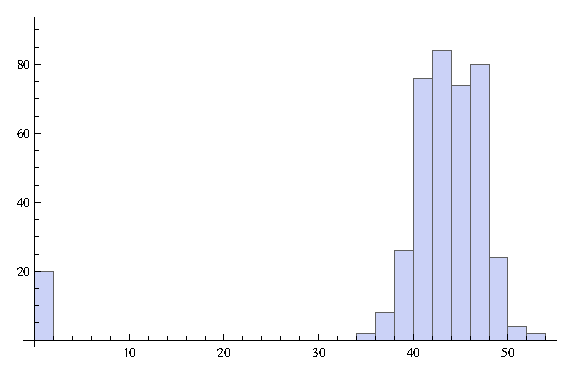
\includegraphics[height=5cm]{1_gr1.eps}
        \end{center}
        When $k = 50$, the answer is 1.71877
        \begin{center}
            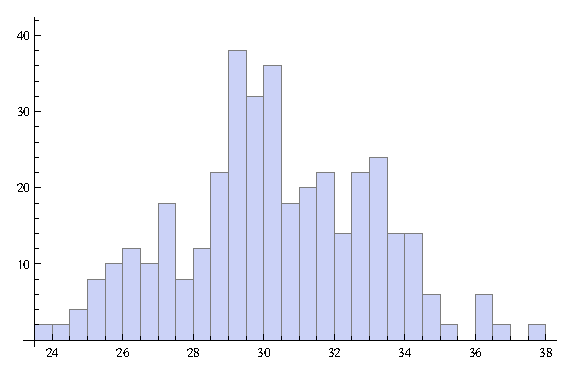
\includegraphics[height=5cm]{1_gr2.eps}
        \end{center}
        When $k = 10$, the answer is 8.20201
        \begin{center}
            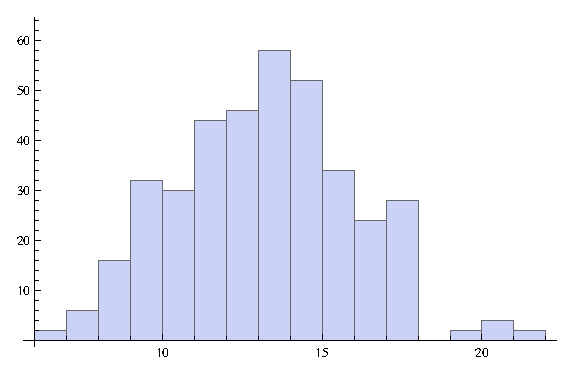
\includegraphics[height=5cm]{1_gr3.eps}
        \end{center}
        When $k = 5$, the answer is 16.6067
        \begin{center}
            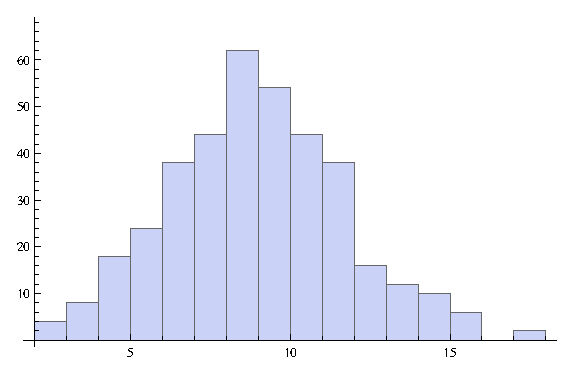
\includegraphics[height=5cm]{1_gr4.eps}
        \end{center}
        When $k = 4$, the answer is 19.3611
        \begin{center}
            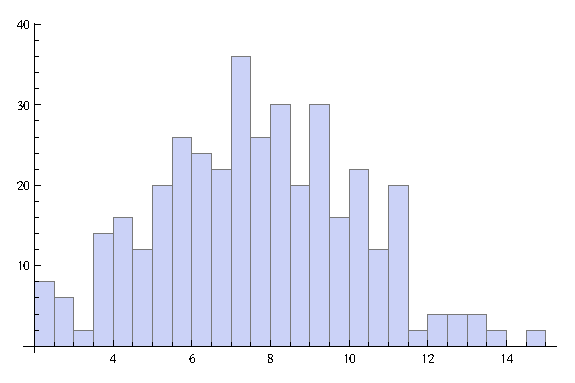
\includegraphics[height=5cm]{1_gr5.eps}
        \end{center}
        When $k = 3$, the answer is 24.5451
        \begin{center}
            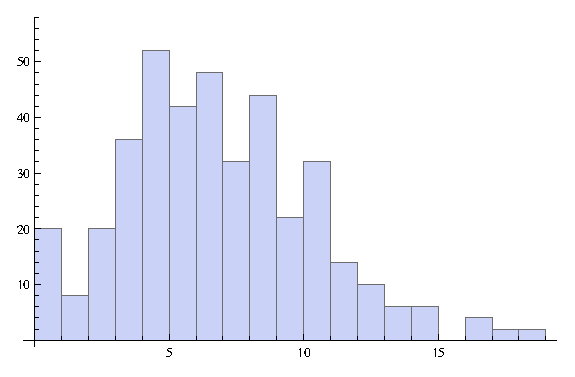
\includegraphics[height=5cm]{1_gr6.eps}
        \end{center}
        When $k = 2$, the answer is 39.0224
        \begin{center}
            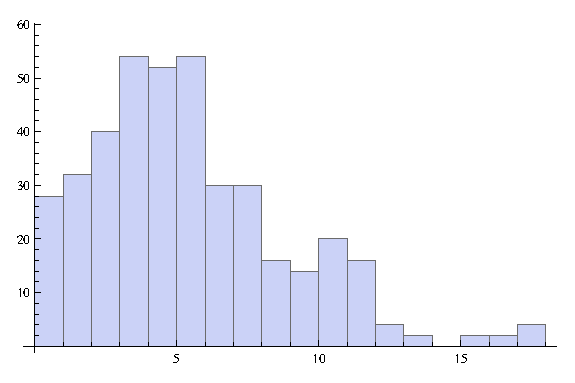
\includegraphics[height=5cm]{1_gr7.eps}
        \end{center}
        When $k = 1$, the answer is 75.2894
        \begin{center}
            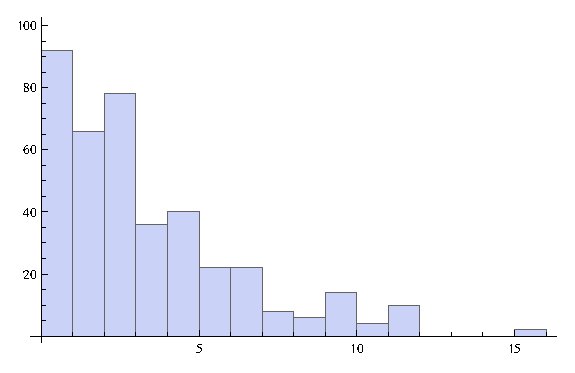
\includegraphics[height=5cm]{1_gr8.eps}
        \end{center}
        As we can see, when the dimension which be projected to goes lower and lower, the relative error goes higher and higher, which is as we expected.
    \end{solution}
\end{enumerate}
\end{document}
